
\tikzset{every picture/.style={line width=0.75pt}} %set default line width to 0.75pt        

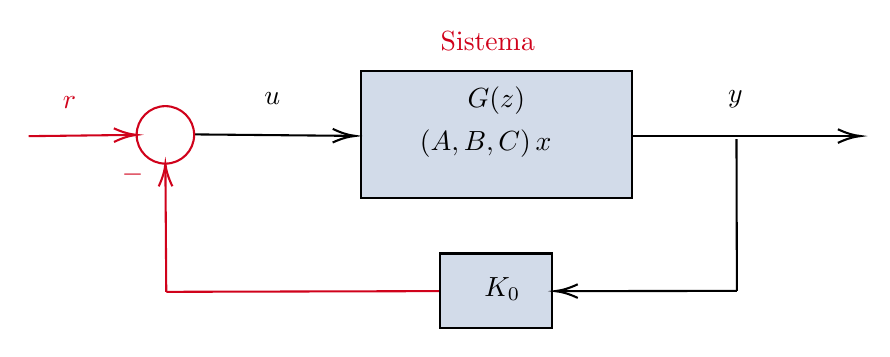
\begin{tikzpicture}[x=0.75pt,y=0.75pt,yscale=-1,xscale=1]
%uncomment if require: \path (0,300); %set diagram left start at 0, and has height of 300

%Shape: Rectangle [id:dp7691782418513171] 
\draw  [fill={rgb, 255:red, 158; green, 176; blue, 208 }  ,fill opacity=0.46 ] (270.2,69.5) -- (400.6,69.5) -- (400.6,130.72) -- (270.2,130.72) -- cycle ;
%Straight Lines [id:da6568557179723491] 
\draw    (400.8,100.72) -- (508.8,100.72) ;
\draw [shift={(510.8,100.72)}, rotate = 180] [color={rgb, 255:red, 0; green, 0; blue, 0 }  ][line width=0.75]    (10.93,-3.29) .. controls (6.95,-1.4) and (3.31,-0.3) .. (0,0) .. controls (3.31,0.3) and (6.95,1.4) .. (10.93,3.29)   ;
%Shape: Rectangle [id:dp6409122366284958] 
\draw  [fill={rgb, 255:red, 158; green, 176; blue, 208 }  ,fill opacity=0.46 ] (308,157.3) -- (362,157.3) -- (362,193.3) -- (308,193.3) -- cycle ;
%Straight Lines [id:da06712304236157962] 
\draw    (189.8,99.92) -- (265.4,100.63) ;
\draw [shift={(267.4,100.65)}, rotate = 180.54] [color={rgb, 255:red, 0; green, 0; blue, 0 }  ][line width=0.75]    (10.93,-3.29) .. controls (6.95,-1.4) and (3.31,-0.3) .. (0,0) .. controls (3.31,0.3) and (6.95,1.4) .. (10.93,3.29)   ;
%Straight Lines [id:da3419447652617802] 
\draw    (451,102.2) -- (451.2,175.32) ;
%Straight Lines [id:da583695130934452] 
\draw    (451.2,175.32) -- (365.6,175.43) ;
\draw [shift={(363.6,175.43)}, rotate = 359.93] [color={rgb, 255:red, 0; green, 0; blue, 0 }  ][line width=0.75]    (10.93,-3.29) .. controls (6.95,-1.4) and (3.31,-0.3) .. (0,0) .. controls (3.31,0.3) and (6.95,1.4) .. (10.93,3.29)   ;
%Shape: Circle [id:dp7704428899101905] 
\draw  [color={rgb, 255:red, 208; green, 2; blue, 27 }  ,draw opacity=1 ] (162,100.15) .. controls (162,92.5) and (168.2,86.3) .. (175.85,86.3) .. controls (183.5,86.3) and (189.7,92.5) .. (189.7,100.15) .. controls (189.7,107.8) and (183.5,114) .. (175.85,114) .. controls (168.2,114) and (162,107.8) .. (162,100.15) -- cycle ;
%Straight Lines [id:da5526597244895324] 
\draw [color={rgb, 255:red, 208; green, 2; blue, 27 }  ,draw opacity=1 ]   (176.27,175.77) -- (307.6,175.43) ;
%Straight Lines [id:da2893181473633277] 
\draw [color={rgb, 255:red, 208; green, 2; blue, 27 }  ,draw opacity=1 ]   (176.27,175.77) -- (175.86,116) ;
\draw [shift={(175.85,114)}, rotate = 449.61] [color={rgb, 255:red, 208; green, 2; blue, 27 }  ,draw opacity=1 ][line width=0.75]    (10.93,-3.29) .. controls (6.95,-1.4) and (3.31,-0.3) .. (0,0) .. controls (3.31,0.3) and (6.95,1.4) .. (10.93,3.29)   ;
%Straight Lines [id:da1586663427610986] 
\draw [color={rgb, 255:red, 208; green, 2; blue, 27 }  ,draw opacity=1 ]   (110,100.77) -- (160,100.17) ;
\draw [shift={(162,100.15)}, rotate = 539.3199999999999] [color={rgb, 255:red, 208; green, 2; blue, 27 }  ,draw opacity=1 ][line width=0.75]    (10.93,-3.29) .. controls (6.95,-1.4) and (3.31,-0.3) .. (0,0) .. controls (3.31,0.3) and (6.95,1.4) .. (10.93,3.29)   ;

% Text Node
\draw (320,75.4) node [anchor=north west][inner sep=0.75pt]    {$G(z)$};
% Text Node
\draw (297,96.4) node [anchor=north west][inner sep=0.75pt]    {$\left( A,B ,C\right)\bm{x}$};
% Text Node
\draw (328,167.4) node [anchor=north west][inner sep=0.75pt]    {$K_0$};
% Text Node
\draw (222,78.4) node [anchor=north west][inner sep=0.75pt]    {$\bm{u}$};
% Text Node
\draw (445.5,77.4) node [anchor=north west][inner sep=0.75pt]    {$\bm{y}$};
% Text Node
\draw (307,49) node [anchor=north west][inner sep=0.75pt]  [color={rgb, 255:red, 208; green, 2; blue, 27 }  ,opacity=1 ] [align=left] {Sistema};
% Text Node
\draw (125,80.4) node [anchor=north west][inner sep=0.75pt]  [color={rgb, 255:red, 208; green, 2; blue, 27 }  ,opacity=1 ]  {$r$};
% Text Node
\draw (153.33,113.4) node [anchor=north west][inner sep=0.75pt]  [color={rgb, 255:red, 208; green, 2; blue, 27 }  ,opacity=1 ]  {$-$};


\end{tikzpicture}